% ============================================================
% FEE3411 Control Systems A -- Tutorial sheet, Week 04
% Topic: Block diagrams, signal flow graphs and Mason's rule
%
% ONE source, TWO outputs. The solutions toggle is driven by \jobname,
% so the two PDFs cannot drift apart:
%
%   latexmk -pdf -jobname=week-04-tutorial-questions week-04-tutorial.tex
%   latexmk -pdf -jobname=week-04-tutorial-solutions week-04-tutorial.tex
%
% Needs: ../tex/preamble.tex (this file lives in Tutorials/).
% ============================================================
\documentclass[11pt,a4paper]{article}
\usepackage[margin=25mm]{geometry}
% ============================================================
% FEE3411 Control Systems A -- shared preamble
% Used by both the lecture notes (article) and the slides (beamer).
% ============================================================
\usepackage[T1]{fontenc}
% lmodern gives cleaner PDF fonts but is absent from minimal TeX installs.
% Load it only if present, so this preamble builds anywhere.
\IfFileExists{lmodern.sty}{\usepackage{lmodern}}{}
\usepackage{amsmath,amssymb,amsthm}
\usepackage{graphicx}
\usepackage{booktabs}
\usepackage{siunitx}
\usepackage{tikz}
\usepackage{circuitikz}
\usepackage{pgfplots}
\pgfplotsset{compat=1.18}
\usetikzlibrary{arrows.meta,positioning,calc,decorations.markings,shapes.geometric}
\usepackage[most]{tcolorbox}
\usepackage{xcolor}

% ---- Course colours -------------------------------------------------
\definecolor{fnavy}{HTML}{1F3864}
\definecolor{faccent}{HTML}{2E5E4E}
\definecolor{fflag}{HTML}{9C4221}

% ---- Block-diagram style --------------------------------------------
\tikzset{
  block/.style   = {draw, thick, rectangle, minimum height=2.6em,
                    minimum width=3.2em, align=center},
  sumnode/.style = {draw, thick, circle, inner sep=0pt, minimum size=1.6em},
  pickoff/.style = {fill, circle, inner sep=0pt, minimum size=3pt},
  sig/.style     = {-{Latex[length=2mm]}, thick},
}

% ---- Summing-junction signs -----------------------------------------
% \sumsign{<node>}{<angle>}{<+ or ->} places a sign just outside the circle.
\newcommand{\sumsign}[3]{\node[font=\small] at ($(#1)+(#2:0.5)$) {$#3$};}

% ---- Boxed environments ---------------------------------------------
\newtcolorbox{keyidea}[1][]{colback=fnavy!5,colframe=fnavy,
  fonttitle=\bfseries,title=Key idea,#1}
\newtcolorbox{workedex}[1][]{colback=faccent!5,colframe=faccent,
  fonttitle=\bfseries,title=Worked example,#1}
\newtcolorbox{pitfall}[1][]{colback=fflag!5,colframe=fflag,
  fonttitle=\bfseries,title=Common pitfall,#1}

% ---- Shorthands ------------------------------------------------------
\newcommand{\Lap}{\mathcal{L}}
\newcommand{\jw}{\mathrm{j}\omega}
\newcommand{\wn}{\omega_{n}}
\newcommand{\zt}{\zeta}
\newcommand{\TF}[1]{#1(s)}

% ---- Week title machinery -------------------------------------------
\usepackage{fancyhdr}
\newcommand{\thecoursecode}{FEE3411}
\newcommand{\thecoursename}{Control Systems A}
\newcommand{\wknum}{}
\newcommand{\wktopic}{}
\newcommand{\weeknumber}[1]{\renewcommand{\wknum}{#1}}
\newcommand{\weektopic}[1]{\renewcommand{\wktopic}{#1}}
\newcommand{\weektitle}{%
  \thispagestyle{plain}%
  \begin{center}
    {\large\sffamily\bfseries\color{fnavy}\thecoursecode: \thecoursename}\\[2pt]
    {\Huge\sffamily\bfseries Week \wknum}\\[4pt]
    {\LARGE\sffamily\color{fnavy}\wktopic}\\[6pt]
    \rule{\textwidth}{1.2pt}
  \end{center}\vspace{4pt}%
  \pagestyle{fancy}\fancyhf{}%
  \fancyhead[L]{\footnotesize\color{gray}\thecoursecode\ Week \wknum\ --- \wktopic}%
  \fancyhead[R]{\footnotesize\color{gray}\thepage}%
  \renewcommand{\headrulewidth}{0.4pt}%
}

% ---- Outcomes and reading boxes -------------------------------------
\newenvironment{outcomes}
  {\begin{tcolorbox}[colback=white,colframe=fnavy!60,
      fonttitle=\bfseries,title=By the end of this week you should be able to]
   \begin{itemize}[leftmargin=*]}
  {\end{itemize}\end{tcolorbox}}

\newtcolorbox{readingbox}{colback=gray!5,colframe=gray!50,
  fonttitle=\bfseries,title=Reading}

% enumitem must NOT be loaded under beamer: it overwrites beamer's itemize
% templates and the bullet markers silently disappear. The notes (article) get
% it; the slides (beamer) use beamer's own list machinery instead.
\makeatletter
\@ifclassloaded{beamer}{}{\usepackage{enumitem}}
\makeatother

\usepackage{environ}

% ---- solutions toggle, decided by the job name ----------------------
% NB: xstring's \IfSubStr does NOT work here -- \jobname yields catcode-12
% characters and the comparison silently fails, giving the questions version
% both times. The expl3 string test below is catcode-blind and does work.
\newif\ifsolutions
\ExplSyntaxOn
\tl_set:Nx \l_tmpa_tl { \jobname }
\str_if_in:NnTF \l_tmpa_tl { solutions } { \solutionstrue } { \solutionsfalse }
\ExplSyntaxOff

\newtcolorbox{solbox}[1][]{colback=faccent!4,colframe=faccent!70,
  fonttitle=\bfseries,title=Solution,breakable,#1}
\NewEnviron{solution}{\ifsolutions\begin{solbox}\BODY\end{solbox}\fi}

% ---- question tagging ------------------------------------------------
\newcommand{\inhour}{\hfill{\small\color{faccent}\itshape[in the hour]}}
\newcommand{\athome}{\hfill{\small\color{fflag}\itshape[homework]}}

% Signs on summing junctions: pushed clear of the arrowheads, as in the notes.
\renewcommand{\sumsign}[3]{\node[font=\scriptsize] at ($(#1)+(#2:0.72)$) {$#3$};}

\weeknumber{4}
\weektopic{Tutorial 4 --- Block Diagrams, Signal Flow Graphs and Mason's Rule}

\begin{document}
\weektitle

\begin{center}
\ifsolutions
  {\large\sffamily\bfseries\color{fflag}QUESTIONS AND SOLUTIONS}\\[2pt]
  {\small\itshape Instructor copy --- do not circulate before the tutorial.}
\else
  {\large\sffamily\bfseries\color{fnavy}QUESTION SHEET}
\fi
\end{center}

\bigskip
\noindent
This hour is reduction practice, and then the same diagram taken the other
way. Question~1 is a nested two-loop reduction; Question~2 is an
\emph{overlapping}-loop diagram that needs a pick-off point moved before it
will collapse; Question~3 converts that same diagram to a signal flow graph and
evaluates it with Mason's rule, so you finish the hour having done one system
by both routes and seen the answers agree. The homework extends Mason to a
graph with a non-touching pair of loops, and revisits the canonical form with
an unknown gain.

\smallskip
\noindent
Questions marked \textbf{\color{faccent}[in the hour]} are the ones we work
through together. Those marked \textbf{\color{fflag}[homework]} you do in your
own time --- they are not collected, but the technique is assumed from here on,
and Assignment~2 (issued this week, due Week~6) covers exactly this material.

\smallskip
\noindent
\emph{Preparation:} Week~4 lecture notes, \S1--\S7.

% --------------------------------------------------------------------
\begin{readingbox}
\textbf{Quick reference --- carry these into every question below.}

\smallskip
\begin{minipage}[t]{0.48\textwidth}
\textbf{The three connections}\\[2pt]
\footnotesize
\[
  \text{cascade: } G_1G_2,
  \qquad
  \text{parallel: } G_1\pm G_2
\]
\[
  \text{negative feedback: } \frac{G}{1+GH}
\]
\textbf{Canonical form}
\[
  T=\frac{C}{R}=\frac{G}{1+GH},
  \qquad
  \frac{E}{R}=\frac{1}{1+GH}
\]
\[
  \text{characteristic equation: } 1+GH=0
\]
\textbf{Moving a junction past a block $G$}
\[
  \text{summing junction, against the flow: } \div G
\]
\[
  \text{pick-off point, with the flow: } \times\tfrac{1}{G}
\]
\end{minipage}
\hfill
\begin{minipage}[t]{0.48\textwidth}
\textbf{Mason's gain formula}\\[2pt]
\footnotesize
\[
  T = \frac{\sum_k P_k\Delta_k}{\Delta}
\]
\[
  \Delta = 1-\sum_i L_i
    + \!\!\sum_{\substack{\text{non-touching}\\ \text{pairs}}}\!\! L_iL_j
    - \cdots
\]
$P_k$: gain of the $k$-th forward path.\\
$L_i$: gain of the $i$-th loop, signs included.\\
$\Delta_k$: $\Delta$ with every loop touching path $k$ deleted.\\
Non-touching $=$ sharing \emph{no node}.

\medskip
\textbf{Second-order denominator}
\[
  s^{2}+2\zt\wn s+\wn^{2}
\]
\end{minipage}
\end{readingbox}

% ====================================================================
\section*{Question 1 --- Nested loops: reduce from the inside out \inhour}

Figure~\ref{fig:q1} shows a position servo with an inner rate loop. The
amplifier has gain $G_1=10$, the power stage is $G_2(s)=1/(s+5)$, the shaft
integrates its input so $G_3(s)=1/s$, the rate sensor has gain $H_1=3$, and the
position sensor is a unit-gain potentiometer.

\begin{figure}[htbp]
\centering
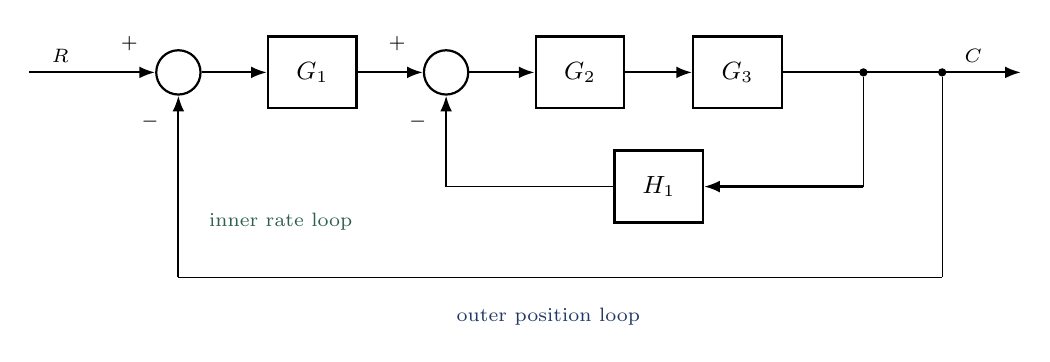
\begin{tikzpicture}[x=1cm,y=1cm,font=\small]
\node[sumnode] (S1) at (1.3,0) {};
\node[block] (A) at (3.0,0) {$G_1$};
\node[sumnode] (S2) at (4.7,0) {};
\node[block] (B) at (6.4,0) {$G_2$};
\node[block] (C) at (8.4,0) {$G_3$};
\node[pickoff] (P1) at (10.0,0) {};
\node[pickoff] (P2) at (11.0,0) {};
\draw[sig] (-0.6,0) -- node[above,font=\scriptsize,pos=0.25]{$R$} (S1);
\draw[sig] (S1) -- (A);
\draw[sig] (A) -- (S2);
\draw[sig] (S2) -- (B);
\draw[sig] (B) -- (C);
\draw[sig] (C) -- (12.0,0) node[above,font=\scriptsize,pos=0.8]{$C$};
% inner rate loop: from output of G3 back to S2 through H1
\node[block] (H1) at (7.4,-1.45) {$H_1$};
\draw (P1) -- (10.0,-1.45); \draw[sig] (10.0,-1.45) -- (H1);
\draw (H1) -- (4.7,-1.45); \draw[sig] (4.7,-1.45) -- (S2);
% outer position loop
\draw (P2) -- (11.0,-2.6); \draw (11.0,-2.6) -- (1.3,-2.6);
\draw[sig] (1.3,-2.6) -- (S1);
\sumsign{S1}{150}{+}
\sumsign{S1}{240}{-}
\sumsign{S2}{150}{+}
\sumsign{S2}{240}{-}
\node[faccent,font=\scriptsize] at (2.6,-1.9) {inner rate loop};
\node[fnavy,font=\scriptsize] at (6.0,-3.1) {outer position loop};
\end{tikzpicture}
\caption{Question 1: a position servo with an inner rate loop.}
\label{fig:q1}
\end{figure}

\begin{enumerate}[label=(\alph*)]
\item Collapse the inner loop to a single block, and say what feedback has
      done to the pole of $G_3$.
\item Cascade the amplifier and power stage with your result, then collapse the
      outer loop to find $T(s)=C(s)/R(s)$.
\item Identify $\wn$ and $\zt$, and give the closed-loop poles.
\item What is the d.c.\ gain of the closed loop? Why is it not $1$, given that
      the forward path contains an integrator?
\end{enumerate}

\begin{solution}
\textbf{(a)} The inner loop is a plain negative-feedback connection of $G_3$
with $H_1$:
\[
  \frac{G_3}{1+G_3H_1}=\frac{\dfrac{1}{s}}{1+\dfrac{3}{s}}=\frac{1}{s+3}.
\]
The free integrator's pole has moved from $s=0$ to $s=-3$: rate feedback has
turned an integrator into a first-order lag with time constant
$\SI{0.333}{\second}$. (It has also, as we shall see in (d), destroyed the
system's ability to follow a step exactly --- there is no free lunch.)

\medskip
\textbf{(b)} Cascading,
\[
  G_1G_2\cdot\frac{1}{s+3}=\frac{10}{(s+3)(s+5)}=\frac{10}{s^{2}+8s+15},
\]
and closing the unity-feedback outer loop,
\[
  T(s)=\frac{\dfrac{10}{s^{2}+8s+15}}{1+\dfrac{10}{s^{2}+8s+15}}
   =\frac{10}{s^{2}+8s+15+10}
   =\frac{10}{s^{2}+8s+25}.
\]

\medskip
\textbf{(c)} Comparing with $s^{2}+2\zt\wn s+\wn^{2}$:
\[
  \wn=\sqrt{25}=\SI{5}{\radian\per\second},
  \qquad
  2\zt\wn=8\;\Longrightarrow\;\zt=\frac{8}{10}=0.8,
\]
and the poles are
\[
  s=-\zt\wn\pm\mathrm{j}\wn\sqrt{1-\zt^{2}}=-4\pm\mathrm{j}3 .
\]
A stable, well-damped pair.

\medskip
\textbf{(d)} $T(0)=10/25=0.4$. The integrator would have given zero
steady-state error \emph{if it had survived}, but the inner rate loop moved its
pole off the origin in part~(a), so the forward path of the outer loop has no
free integrator left and its d.c.\ gain is finite:
$G_1G_2/(s+3)$ at $s=0$ equals $10/15=2/3$, so
$T(0)=(2/3)/(1+2/3)=0.4$. The servo settles $60\%$ short of its reference ---
the price of the extra damping, and exactly the trade-off Week~6 quantifies
with static error constants.
\end{solution}

\begin{pitfall}
It is tempting to write ``the forward path has an integrator, so the d.c.\ gain
is $1$''. That rule belongs to the \emph{outer} loop's forward path, and in
this diagram the integrator is inside the inner loop, where feedback has
already relocated its pole. Always check which loop a block ends up inside
after the first collapse.
\end{pitfall}

% ====================================================================
\section*{Question 2 --- Overlapping loops: move a pick-off point \inhour}

Figure~\ref{fig:q2} has two loops that overlap: loop~1 (through $H_1$) spans
$G_1$ and $G_2$, and loop~2 (through $H_2$) spans $G_2$ and $G_3$. The values
are
\[
  G_1=2,\qquad G_2(s)=\frac{1}{s+1},\qquad G_3(s)=\frac{4}{s+6},
  \qquad H_1=1,\qquad H_2=0.5 .
\]

\begin{figure}[htbp]
\centering
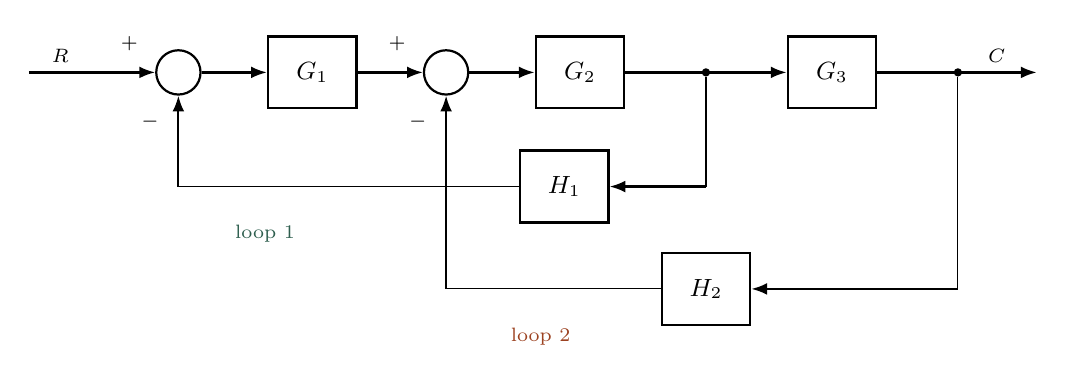
\begin{tikzpicture}[x=1cm,y=1cm,font=\small]
\node[sumnode] (S1) at (1.3,0) {};
\node[block] (G1) at (3.0,0) {$G_1$};
\node[sumnode] (S2) at (4.7,0) {};
\node[block] (G2) at (6.4,0) {$G_2$};
\node[pickoff] (P1) at (8.0,0) {};
\node[block] (G3) at (9.6,0) {$G_3$};
\node[pickoff] (P2) at (11.2,0) {};
\draw[sig] (-0.6,0) -- node[above,font=\scriptsize,pos=0.25]{$R$} (S1);
\draw[sig] (S1) -- (G1);
\draw[sig] (G1) -- (S2);
\draw[sig] (S2) -- (G2);
\draw[sig] (G2) -- (G3);
\draw[sig] (G3) -- (12.2,0) node[above,font=\scriptsize,pos=0.75]{$C$};
% loop 1: from output of G2 back to S1 via H1
\node[block] (H1) at (6.2,-1.45) {$H_1$};
\draw (P1) -- (8.0,-1.45); \draw[sig] (8.0,-1.45) -- (H1);
\draw (H1) -- (1.3,-1.45); \draw[sig] (1.3,-1.45) -- (S1);
% loop 2: from C back to S2 via H2
\node[block] (H2) at (8.0,-2.75) {$H_2$};
\draw (P2) -- (11.2,-2.75); \draw[sig] (11.2,-2.75) -- (H2);
\draw (H2) -- (4.7,-2.75); \draw[sig] (4.7,-2.75) -- (S2);
\sumsign{S1}{150}{+}
\sumsign{S1}{240}{-}
\sumsign{S2}{150}{+}
\sumsign{S2}{240}{-}
\node[faccent,font=\scriptsize] at (2.4,-2.05) {loop 1};
\node[fflag,font=\scriptsize] at (5.9,-3.35) {loop 2};
\end{tikzpicture}
\caption{Question 2: overlapping loops. Loop~1 spans $G_1,G_2$ and loop~2
spans $G_2,G_3$ --- neither contains the other.}
\label{fig:q2}
\end{figure}

\begin{enumerate}[label=(\alph*)]
\item Explain in one sentence why this diagram cannot be reduced by collapsing
      an inner loop first.
\item Move loop~1's pick-off point forward through $G_3$, stating the gain the
      moved branch must now carry.
\item Reduce the resulting nested diagram to find $T(s)=C(s)/R(s)$, in factored
      form.
\item State the closed-loop poles and the d.c.\ gain.
\end{enumerate}

\begin{solution}
\textbf{(a)} Neither loop lies inside the other --- they share only $G_2$ ---
so there is no innermost loop to collapse, and the feedback formula cannot be
applied to either one on its own.

\medskip
\textbf{(b)} Loop~1 is fed from the output of $G_2$. Moving that pick-off
forward through $G_3$ means the branch now taps $G_3$ times the old signal, so
it must be compensated by $1/G_3$:
\[
  H_1 \;\longrightarrow\; \frac{H_1}{G_3}=\frac{1}{4/(s+6)}=\frac{s+6}{4}.
\]
Loop~1 now taps the same node as loop~2, and loop~2 sits inside it: the loops
are nested.

\medskip
\textbf{(c)} Collapse the inner loop ($G_2G_3$ with $H_2$) first:
\[
  \frac{G_2G_3}{1+G_2G_3H_2}
  =\frac{\dfrac{4}{(s+1)(s+6)}}{1+\dfrac{2}{(s+1)(s+6)}}
  =\frac{4}{(s+1)(s+6)+2}
  =\frac{4}{s^{2}+7s+8}.
\]
The outer loop now has forward path $G_1\times$ that, and feedback path
$(s+6)/4$:
\[
  T(s)=\frac{\dfrac{8}{s^{2}+7s+8}}
            {1+\dfrac{8}{s^{2}+7s+8}\cdot\dfrac{s+6}{4}}
   =\frac{8}{s^{2}+7s+8+2(s+6)} ,
\]
so
\[
  T(s)=\frac{8}{s^{2}+9s+20}=\frac{8}{(s+4)(s+5)} .
\]

\medskip
\textbf{(d)} Poles at $s=-4$ and $s=-5$: real, distinct, stable. D.c.\ gain
$T(0)=8/20=0.4$. Note that the \emph{open-loop} poles were $-1$ and $-6$;
feedback has pulled them together into $-4$ and $-5$.
\end{solution}

% ====================================================================
\section*{Question 3 --- The same system, by SFG and Mason \inhour}

Now take the \emph{original} diagram of Figure~\ref{fig:q2} --- before any
junction was moved --- and evaluate it the other way.

\begin{enumerate}[label=(\alph*)]
\item Draw the signal flow graph. Use nodes $R$, $E_1$ (the output of the first
      summing junction), $E_2$ (the output of the second), $X$ (the output of
      $G_2$) and $C$.
\item List every forward path with its gain, and every loop with its loop gain.
      Are the two loops touching or non-touching? Justify your answer by
      listing each loop's nodes.
\item Write down $\Delta$ and the cofactor $\Delta_1$, and evaluate Mason's
      formula.
\item Compare with your answer to Question~2(c). What have you gained, and
      what have you lost, by using Mason's rule instead of reduction?
\end{enumerate}

\begin{solution}
\textbf{(a)} The graph is drawn below. Each summing junction has become a
node, and the two feedback signs have been absorbed into the branch gains
$-H_1$ and $-H_2$.

\begin{center}
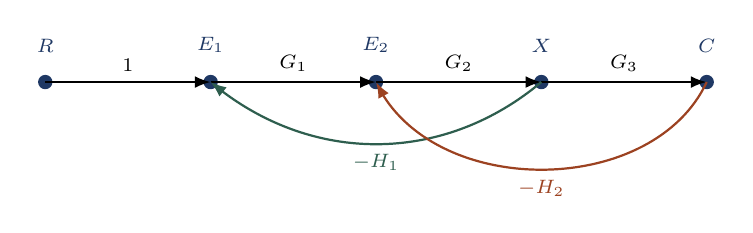
\begin{tikzpicture}[x=1cm,y=1cm,font=\small]
\foreach \x/\lab in {0/$R$, 2.1/$E_1$, 4.2/$E_2$, 6.3/$X$, 8.4/$C$}{
  \fill[fnavy] (\x,0) circle (2.6pt);
  \node[fnavy,font=\scriptsize,above=7pt] at (\x,0) {\lab};}
\draw[sig] (0,0) -- node[above,font=\scriptsize]{$1$} (2.1,0);
\draw[sig] (2.1,0) -- node[above,font=\scriptsize]{$G_1$} (4.2,0);
\draw[sig] (4.2,0) -- node[above,font=\scriptsize]{$G_2$} (6.3,0);
\draw[sig] (6.3,0) -- node[above,font=\scriptsize]{$G_3$} (8.4,0);
% loop 1: X back to E1
\draw[sig,faccent] (6.3,0) to[out=-140,in=-40] node[below,font=\scriptsize,pos=0.5]{$-H_1$} (2.1,0);
% loop 2: C back to E2
\draw[sig,fflag] (8.4,0) to[out=-115,in=-65] node[below,font=\scriptsize,pos=0.5]{$-H_2$} (4.2,0);
\end{tikzpicture}\\[4pt]
{\footnotesize The signal flow graph of Figure~\ref{fig:q2}.}
\end{center}

\medskip
\textbf{(b)} One forward path:
\[
  P_1 = G_1G_2G_3 = 2\cdot\frac{1}{s+1}\cdot\frac{4}{s+6}
      = \frac{8}{(s+1)(s+6)} .
\]
Two loops:
\[
  L_1 = -G_1G_2H_1 = -\frac{2}{s+1},
  \qquad
  L_2 = -G_2G_3H_2 = -\frac{2}{(s+1)(s+6)} .
\]
Loop~1 visits $E_1, E_2, X$; loop~2 visits $E_2, X, C$. The sets share $E_2$
and $X$, so the loops are \textbf{touching} --- there is no non-touching pair,
and $\Delta$ stops after the loop-gain sum.

\medskip
\textbf{(c)}
\[
  \Delta = 1-(L_1+L_2) = 1+\frac{2}{s+1}+\frac{2}{(s+1)(s+6)},
  \qquad \Delta_1 = 1,
\]
($\Delta_1=1$ because the forward path passes through both loops). Multiplying
numerator and denominator by $(s+1)(s+6)$,
\[
  T(s)=\frac{P_1\Delta_1}{\Delta}
   =\frac{8}{(s+1)(s+6)+2(s+6)+2}
   =\frac{8}{s^{2}+9s+20}
   =\frac{8}{(s+4)(s+5)} ,
\]
identical to Question~2(c).

\medskip
\textbf{(d)} Gained: no junction was moved, no diagram was redrawn, and no
intermediate transfer function had to be carried --- three fewer places to make
a slip. Lost: the intermediate results themselves. Question~2 revealed on the
way that the inner loop alone is $4/(s^{2}+7s+8)$, which is the transfer
function you would need if you were asked about the signal at $C$ with loop~1
disconnected. Mason gives the end-to-end answer and nothing else.
\end{solution}

\begin{keyidea}
Doing one system both ways, as Questions~2 and~3 just did, is the best
available check on a reduction. If the two routes disagree, the error is
almost always a lost sign at a summing junction or a forgotten compensating
factor on a moved branch --- look there first, not at the arithmetic.
\end{keyidea}

% ====================================================================
\section*{Question 4 --- Mason with a non-touching pair \athome}

Figure~\ref{fig:q4} is a signal flow graph with a feedforward branch. Take
\[
  a_1=2,\quad a_2(s)=\frac{1}{s+1},\quad a_3(s)=\frac{4}{s+2},\quad a_4=1,
  \quad a_5=0.5,\quad b_1=1,\quad b_2=1 .
\]

\begin{figure}[htbp]
\centering
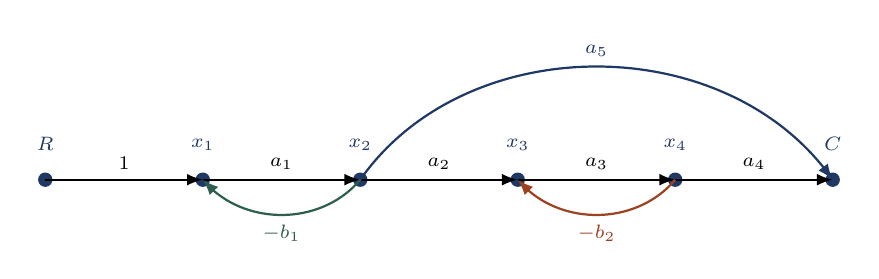
\begin{tikzpicture}[x=1cm,y=1cm,font=\small]
\foreach \x/\lab in {0/$R$, 2.0/$x_1$, 4.0/$x_2$, 6.0/$x_3$, 8.0/$x_4$, 10.0/$C$}{
  \fill[fnavy] (\x,0) circle (2.6pt);
  \node[fnavy,font=\scriptsize,above=7pt] at (\x,0) {\lab};}
\draw[sig] (0,0) -- node[above,font=\scriptsize]{$1$} (2.0,0);
\draw[sig] (2.0,0) -- node[above,font=\scriptsize]{$a_1$} (4.0,0);
\draw[sig] (4.0,0) -- node[above,font=\scriptsize]{$a_2$} (6.0,0);
\draw[sig] (6.0,0) -- node[above,font=\scriptsize]{$a_3$} (8.0,0);
\draw[sig] (8.0,0) -- node[above,font=\scriptsize]{$a_4$} (10.0,0);
% feedforward branch x2 -> C, above the chain
\draw[sig,fnavy] (4.0,0) to[out=55,in=125] node[above,font=\scriptsize,pos=0.5]{$a_5$} (10.0,0);
% loops
\draw[sig,faccent] (4.0,0) to[out=-130,in=-50] node[below,font=\scriptsize]{$-b_1$} (2.0,0);
\draw[sig,fflag] (8.0,0) to[out=-130,in=-50] node[below,font=\scriptsize]{$-b_2$} (6.0,0);
\end{tikzpicture}
\caption{Question 4: a graph with two forward paths and two loops.}
\label{fig:q4}
\end{figure}

\begin{enumerate}[label=(\alph*)]
\item Identify both forward paths and both loops, with their gains.
\item Show that the two loops are non-touching, and hence write down $\Delta$.
\item Show that your $\Delta$ factors as $(1-L_1)(1-L_2)$. Explain why this
      factorisation is guaranteed whenever the graph's only two loops are
      non-touching.
\item Find both cofactors $\Delta_1$ and $\Delta_2$, and hence $T(s)=C/R$.
\item State the closed-loop poles and the d.c.\ gain. Where did the numerator's
      zeros come from --- and would they be there if $a_5$ were removed?
\end{enumerate}

\begin{solution}
\textbf{(a)} Two forward paths:
\[
  P_1 = a_1a_2a_3a_4 = 2\cdot\frac{1}{s+1}\cdot\frac{4}{s+2}\cdot 1
      = \frac{8}{(s+1)(s+2)},
  \qquad
  P_2 = a_1a_5 = 2(0.5) = 1 ,
\]
the second running $R\to x_1\to x_2\to C$ along the feedforward branch. Two
loops:
\[
  L_1 = -a_1b_1 = -2 \quad (x_1,x_2),
  \qquad
  L_2 = -a_3b_2 = -\frac{4}{s+2} \quad (x_3,x_4).
\]

\medskip
\textbf{(b)} Loop~1 visits $x_1$ and $x_2$; loop~2 visits $x_3$ and $x_4$. The
two node sets are disjoint, so the loops are non-touching and $\Delta$ carries
their product:
\[
  \Delta = 1-(L_1+L_2)+L_1L_2
   = 1+2+\frac{4}{s+2}+\frac{8}{s+2}
   = 3+\frac{12}{s+2}
   = \frac{3(s+6)}{s+2} .
\]

\medskip
\textbf{(c)} Directly,
\[
  (1-L_1)(1-L_2) = (1+2)\left(1+\frac{4}{s+2}\right)
   = 3\cdot\frac{s+6}{s+2} = \frac{3(s+6)}{s+2} = \Delta . \checkmark
\]
It is guaranteed because $(1-L_1)(1-L_2)=1-L_1-L_2+L_1L_2$ is \emph{exactly}
Mason's $\Delta$ when the only two loops present do not touch: the
non-touching-pair term supplies the cross product that completes the
factorisation. With touching loops the $L_1L_2$ term is absent and $\Delta$
does not factor this way.

\medskip
\textbf{(d)} $P_1$ runs through all four of $x_1,x_2,x_3,x_4$, so it touches
both loops and $\Delta_1=1$. $P_2$ leaves the chain at $x_2$: it touches
loop~1 but not loop~2, so loop~2 survives in its cofactor,
\[
  \Delta_2 = 1-L_2 = 1+\frac{4}{s+2}=\frac{s+6}{s+2} .
\]
Hence
\[
  T(s)=\frac{P_1\Delta_1+P_2\Delta_2}{\Delta}
   =\frac{\dfrac{8}{(s+1)(s+2)}+\dfrac{s+6}{s+2}}{\dfrac{3(s+6)}{s+2}} ,
\]
and multiplying numerator and denominator by $(s+1)(s+2)$,
\[
  T(s)=\frac{8+(s+6)(s+1)}{3(s+6)(s+1)}
   =\frac{s^{2}+7s+14}{3(s+1)(s+6)} .
\]

\medskip
\textbf{(e)} Poles at $s=-1$ and $s=-6$; d.c.\ gain
$T(0)=14/(3\cdot 6)=7/9\approx0.78$. The numerator's roots are
$s=-3.5\pm\mathrm{j}1.32$ --- a complex pair of zeros, contributed entirely by
the feedforward branch. With $a_5=0$ the second forward path disappears,
$T$ collapses to $P_1/\Delta = 8/[3(s+1)(s+6)]$, and the zeros go with it.
A parallel route through a system puts zeros in its transfer function; this is
Week~3's lesson arriving from the block-diagram side.
\end{solution}

\begin{pitfall}
The commonest error in this question is writing $\Delta_2=1$ out of habit. A
cofactor is $1$ only when the path touches \emph{every} loop. Before writing
$\Delta_k$, list the nodes on path $k$ and strike out only the loops that share
one --- here that is loop~1 alone, which is why loop~2 stays in $\Delta_2$.
\end{pitfall}

% ====================================================================
\section*{Question 5 --- The canonical form with an unknown gain \athome}

A unity-feedback system has forward path
\[
  G(s)=\frac{K}{s(s+5)},\qquad K>0 .
\]

\begin{enumerate}[label=(\alph*)]
\item Write down the open-loop transfer function, the characteristic equation
      and the closed-loop transfer function $T(s)$ in terms of $K$.
\item Find the value of $K$ that gives a natural frequency
      $\wn=\SI{4}{\radian\per\second}$, and the damping ratio $\zt$ that comes
      with it.
\item Give the closed-loop poles for that $K$.
\item Find the steady-state error to a unit step, using $E(s)/R(s)$. Explain
      the answer in one sentence.
\item If $K$ is raised to $64$, what happens to $\wn$ and $\zt$? State the
      general relationship between $K$ and $\zt$ for this system, and say what
      it implies about raising gain to make a system faster.
\end{enumerate}

\begin{solution}
\textbf{(a)} Open loop $G(s)H(s)=K/[s(s+5)]$ (since $H=1$); characteristic
equation
\[
  1+\frac{K}{s(s+5)}=0
  \quad\Longleftrightarrow\quad
  s^{2}+5s+K=0 ;
\]
and
\[
  T(s)=\frac{G}{1+G}=\frac{K}{s(s+5)+K}=\frac{K}{s^{2}+5s+K} .
\]

\medskip
\textbf{(b)} Matching $s^{2}+5s+K$ to $s^{2}+2\zt\wn s+\wn^{2}$ gives
$\wn=\sqrt{K}$ and $2\zt\wn=5$. So $\wn=4$ requires
\[
  K=\wn^{2}=16,
  \qquad
  \zt=\frac{5}{2\wn}=\frac{5}{8}=0.625 .
\]

\medskip
\textbf{(c)} $T(s)=16/(s^{2}+5s+16)$, and
\[
  s=-\zt\wn\pm\mathrm{j}\wn\sqrt{1-\zt^{2}}
   =-2.5\pm\mathrm{j}3.12 .
\]

\medskip
\textbf{(d)} With $K=16$,
\[
  \frac{E(s)}{R(s)}=\frac{1}{1+G}=\frac{s(s+5)}{s^{2}+5s+16},
  \qquad
  e_{ss}=\lim_{s\to0}s\cdot\frac{s(s+5)}{s^{2}+5s+16}\cdot\frac{1}{s}=0 .
\]
The error is zero because the forward path contains a free integrator, which
drives the error to nothing at steady state --- the result Week~6 states as
``a type-1 system has zero steady-state error to a step''.

\medskip
\textbf{(e)} At $K=64$: $\wn=\sqrt{64}=\SI{8}{\radian\per\second}$ and
$\zt=5/(2\cdot8)=5/16=0.3125$. In general
\[
  \wn=\sqrt{K},\qquad \zt=\frac{5}{2\sqrt{K}} \;\propto\; \frac{1}{\sqrt{K}} ,
\]
so raising the gain speeds the system up ($\wn$ rises) but \emph{always} at the
cost of damping ($\zt$ falls): the response gets faster and more oscillatory
together. Gain alone cannot buy both. Week~8 draws this trade-off as the root
locus, and FEE3412 breaks the compromise by changing the shape of $G(s)$ rather
than just its size --- which is what a compensator is for.
\end{solution}

% ====================================================================
\section*{Question 6 --- Two inputs, one characteristic equation \athome}

In Figure~\ref{fig:q6} the reference is $R$, and $U$ is a second input entering
between the two forward blocks. Take $G_a=5$, $G_b(s)=1/(s+3)$ and unity
feedback.

\begin{figure}[htbp]
\centering
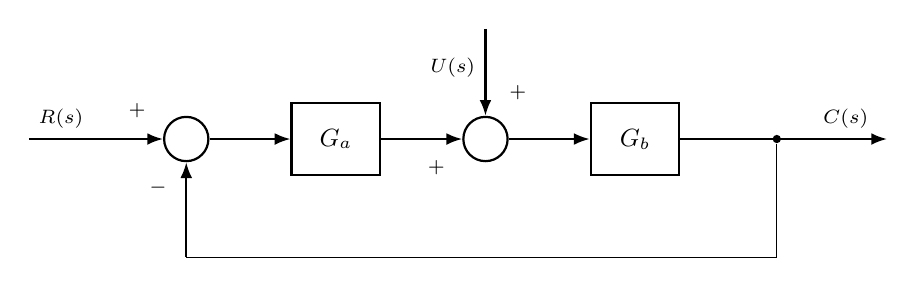
\begin{tikzpicture}[x=1cm,y=1cm,font=\small]
\node[sumnode] (S1) at (1.5,0) {};
\node[block] (G1) at (3.4,0) {$G_a$};
\node[sumnode] (S2) at (5.3,0) {};
\node[block] (G2) at (7.2,0) {$G_b$};
\node[pickoff] (P) at (9.0,0) {};
\draw[sig] (-0.5,0) -- node[above,font=\scriptsize,pos=0.24]{$R(s)$} (S1);
\draw[sig] (S1) -- (G1);
\draw[sig] (G1) -- (S2);
\draw[sig] (S2) -- (G2);
\draw[sig] (G2) -- (10.4,0) node[above,font=\scriptsize,pos=0.8]{$C(s)$};
\draw[sig] (5.3,1.4) -- node[left,font=\scriptsize,pos=0.45]{$U(s)$} (S2);
\draw (P) -- (9.0,-1.5); \draw (9.0,-1.5) -- (1.5,-1.5);
\draw[sig] (1.5,-1.5) -- (S1);
\sumsign{S1}{150}{+}
\sumsign{S1}{240}{-}
\sumsign{S2}{210}{+}
\sumsign{S2}{55}{+}
\end{tikzpicture}
\caption{Question 6: a system with a second input entering after $G_a$.}
\label{fig:q6}
\end{figure}

\begin{enumerate}[label=(\alph*)]
\item Find $C(s)/R(s)$ with $U=0$, and $C(s)/U(s)$ with $R=0$.
\item Write the total response $C(s)$ in terms of both inputs.
\item Why do the two transfer functions have the same denominator?
\item $R$ is a unit step and $U$ is a constant $-2$ (a steady load pulling the
      output down). Find the steady-state value of $c(t)$.
\item What constant value of $U$ would hold the output at zero in the steady
      state while the unit step at $R$ is still applied?
\end{enumerate}

\begin{solution}
\textbf{(a)} With $U=0$ the diagram is the canonical form with forward path
$G_aG_b=5/(s+3)$:
\[
  \frac{C}{R}=\frac{G_aG_b}{1+G_aG_b}
   =\frac{\dfrac{5}{s+3}}{1+\dfrac{5}{s+3}}
   =\frac{5}{s+8} .
\]
With $R=0$, the input $U$ sees only $G_b$ on the way out but the same loop on
the way round:
\[
  \frac{C}{U}=\frac{G_b}{1+G_aG_b}
   =\frac{\dfrac{1}{s+3}}{1+\dfrac{5}{s+3}}
   =\frac{1}{s+8} .
\]

\medskip
\textbf{(b)} By superposition,
\[
  C(s)=\frac{5}{s+8}R(s)+\frac{1}{s+8}U(s) .
\]

\medskip
\textbf{(c)} Because both are governed by the same loop, and so by the same
characteristic equation $1+G_aG_b=0$, i.e.\ $s+8=0$. The poles belong to the
loop, not to the input; an extra input can only change the numerator. (This is
why $U$'s contribution is exactly one fifth of $R$'s here: it misses $G_a=5$ on
the way out.)

\medskip
\textbf{(d)} With $R(s)=1/s$ and $U(s)=-2/s$,
\[
  C(s)=\frac{5}{s+8}\cdot\frac{1}{s}+\frac{1}{s+8}\cdot\frac{-2}{s},
\]
and by the final value theorem (both terms' poles are at $-8$, in the left half
plane, so it applies)
\[
  c(\infty)=\lim_{s\to0}sC(s)=\frac{5}{8}-\frac{2}{8}=\frac{3}{8}=0.375 .
\]

\medskip
\textbf{(e)} Setting the steady-state sum to zero with $R$ a unit step,
\[
  \frac{5}{8}+\frac{u}{8}=0 \quad\Longrightarrow\quad u=-5 .
\]
A constant $U=-5$ exactly cancels a unit step at $R$ at steady state --- which
is worth noticing: a disturbance entering \emph{after} the amplifier needs to
be $G_a$ times larger than the reference to do equal damage, which is precisely
why loop gain ahead of the disturbance point is what protects a system. Using
that observation to \emph{design} the loop is FEE3412's business; computing the
response, as here, is ours.
\end{solution}

% ====================================================================
\vfill
\begin{center}
\rule{0.5\textwidth}{0.4pt}\\[4pt]
{\small\itshape
\ifsolutions
  End of solutions. Week~5: transient response of first- and second-order
  systems.
\else
  Solutions to the homework questions are released with the Week~5 sheet.\\
  Next week: transient response of first- and second-order systems.
\fi}
\end{center}

\end{document}
